\documentclass{article}

\usepackage{fontspec}
\usepackage[russian,english]{babel}
\usepackage{amsmath}
\usepackage{mathtools}
\usepackage{minted}
\usepackage{filecontents}
\usepackage{biblatex}

\setmainfont{CMU Serif}

\title{Отчёт: задача о полёте на максимальную дальность}
\author{Serge Kozlukov\\ \texttt{newkozlukov [at] gmail [dot] com}}

\begin{filecontents}{farthest-flight.bib}
  @misc{katsaran1,
    title={Метод малого параметра в задачах оптимального управления},
    author={Кацаран~Т.~.К.,\ Кабанцова~Л.~Ю.},
    city={Воронеж},
    publisher={Издательский дом ``ВГУ''},
    year=2016,
    }
\end{filecontents}

\addbibresource{farthest-flight.bib}

\begin{document}
\thispagestyle{empty}
\begin{center}
МИНИСТЕРСТВО ОБРАЗОВАНИЯ И НАУКИ РОССИЙСКОЙ ФЕДЕРАЦИИ,\\
ФЕДЕРАЛЬНОЕ ГОСУДАРСТВЕННОЕ БЮДЖЕТНОЕ ОБРАЗОВАТЕЛЬНОЕ
УЧЕРЕЖДЕНИЕ ВЫСШЕГО ОБРАЗОВАНИЯ\\
``ВОРОНЕЖСКИЙ ГОСУДАРСТВЕННЫЙ УНИВЕРСИТЕТ''\\
(ФГБОУ ВО ``ВГУ''),\\
ФАКУЛЬТЕТ ПРИКЛАДНОЙ МАТЕМАТИКИ, ИНФОРМАТИКИ И МЕХАНИКИ,\\
КАФЕДРА НЕЛИНЕЙНЫХ КОЛЕБАНИЙ
\end{center}
\vfill
\begin{center}
  \textbf{ОТЧЁТ}\\[1.5cm]
  по лабораторной работе\\
  ``Задача о полёте на максимальную дальность''\\
  по специальности 01.03.02 ``Прикладная Математика, Механика и Информатика''
\end{center}
\vfill
\begin{flushright}
  Выполнил:\\
  Студент 4 курса, 6 группы\\
  Сергей Викторович Козлуков.\\
  Проверил(а):\\
  доц. Кацаран Т.~К.
\end{flushright}
\begin{center}
  Воронеж\\2018
\end{center}

\clearpage
\tableofcontents

\section{Постановка задачи}
Рассмотрим летательный аппарт, не имеющий двигателя, управляемый с помощью
изменения площади несущей поверхности \( S \) и угла атаки \( \alpha \).
Требуется найти управление \(t\mapsto S, \alpha\), максимизирующее дальность полёта.

Эволюция системы описывается~\cite{katsaran1} задачей Коши:
\begin{equation}
  \left\{
    \begin{aligned}
      & m\ddot x_1(t) = - R(t)\cos\theta - Y(t)\sin\theta,\\
      & m\ddot x_2(t) = - mg - R(t)\sin\theta - Y(t)\cos\theta,\\
      & x_1(t_0) = x_2(t_0) = 0,\\
      & \dot x_1(t_0) = |V_0|\cos\theta,\\
      & \dot x_2(t_0) = |V_0|\sin\theta,
      \end{aligned}
  \right.
\end{equation}
где
\[ R(t) = \frac12 \rho V(t)^2 S(t) C_x,\]
\[ Y(t) = \frac12 \rho V(t)^2 S(t) C_y.\]

Вводя малый параметр
\[ \varepsilon = \frac{V_0^2}{2mg}, \]
и понижая степень уравнения, получим систему:
\begin{equation}
  \left\{
    \begin{aligned}
      & \dot x_1(t) = x_3(t),\\
      & \dot x_2(t) = x_4(t),\\
      & \dot x_3(t) = -\varepsilon\rho V(t)S(t) (C_x(\alpha(t)) x_3(t) + C_y(\alpha(t)) x_4(t)),\\
      & \dot x_4(t) = -1 + \varepsilon V(t)S(t) (C_x(\alpha(t)) x_4(t) - C_y(\alpha(t)) x_3(t)),\\
      & x_1(t_0) = 0,\\
      & x_2(t_0) = 0,\\
      & x_3(t_0) = |V_0|\cos\theta,\\
      & x_4(t_0) = |V_0|\sin\theta,\\
      & -x_1(T) \to\inf.
    \end{aligned}
  \right.
\end{equation}
Из условия оптимальности получим:
\[
  \alpha(t) = \frac12 \arctan(K\tan2\alpha_0\frac{\cos\theta_0 +
    t\sin\theta_0}{\sin2\theta_0 - t\cos\theta_0}),
\]
\[
  S(t) = \left\{ \begin{aligned}
      & S_1,\ \text{if}\ \alpha < \alpha_0,\\
      & S_2,\ \alpha\geq\alpha_0,
    \end{aligned} \right.
\]
\[
  C_x(\alpha) = 1 - \cos\alpha_0\cos\alpha,\\
\]
\[
  C_y(\alpha) = K\sin2\alpha_0\sin2\alpha.
\]

\section{Численная реализация}

\begin{minted}{python}
@attr.s
class FarhestFlight:
    theta0 = attr.ib(np.pi/4)  # attack angle
    alpha0 = attr.ib(np.pi/6)  # idk...
    K = attr.ib(3.5) # capacity
    rho = attr.ib(1.2) # normalized density
    v0 = attr.ib(.8) # normalized initial speed
    S1 = attr.ib(1.0) # support surface area
    S2 = attr.ib(1.5)
    m = attr.ib(1.) # mass
    g = attr.ib(9.8)
    vareps = attr.ib(attr.Factory(
        lambda self: self.v0**2/(2*self.m*self.g),
        takes_self=True))
    
    def ini(self):
        return np.array([
            0,
            0,
            self.v0 * np.cos(self.theta0),
            self.v0 * np.sin(self.theta0)])
    @remove_discontinuity(t0=1)
    def _alpha_arctan_arg(self, t):
        return (
            self.K
            * np.tan(2*self.alpha0)
            * (np.cos(2*self.theta0) + t*np.sin(self.theta0))
            / (np.sin(self.theta0) - t*np.cos(self.theta0)))
    def alpha(self, t):
        return 0.5 * np.arctan(self._alpha_arctan_arg(t))
    def CxCy(self, alpha):
        return np.array([
            1 - np.cos(2*self.alpha0) * np.cos(2*alpha),
            self.K * np.sin(2*self.alpha0)*np.sin(2*alpha)
        ])
    def flow(self, t, y):
        x1, x2, x3, x4 = y
        velo = np.linalg.norm([x3, x4])
        vareps = self.vareps
        a = self.alpha(t)
        S = self.S1 if a < self.alpha0 else self.S2
        Cx, Cy = self.CxCy(a)
        R = .5 * self.rho * (velo**2) * S * Cx
        Y = .5 * self.rho * (velo**2) * S * Cy
        return np.array([
            x3,
            x4,
            -vareps*self.rho*velo*S*(Cx*x3 + Cy*x4),
            -1 + vareps*self.rho*velo*S*(Cx*x3 - Cy*x4)
        ])


t0, t1 = 0, 10
end_of_flight = lambda t, y: y[1] - 0 if y[0] > .001 else 1
end_of_flight.terminal = True
control_switch = lambda t, y: ivp.alpha(t) - ivp.alpha0
sol = scipy.integrate.solve_ivp(ivp.flow, (t0, t1), ivp.ini(),
                                max_step=.001,
                                events=[end_of_flight,
                                        control_switch])
                                      
def plot(x, y, legend):
    p = plt.figure()
    p.line(x, y, legend=legend)
    p.vbar(sol.t_events[1], .001, np.max(y), np.min(y),
           legend='control switch', color='red')
    plt.show(p)


plot(sol.t, sol.y[2, :], legend='\\dot x over time')
\end{minted}

\begin{center}
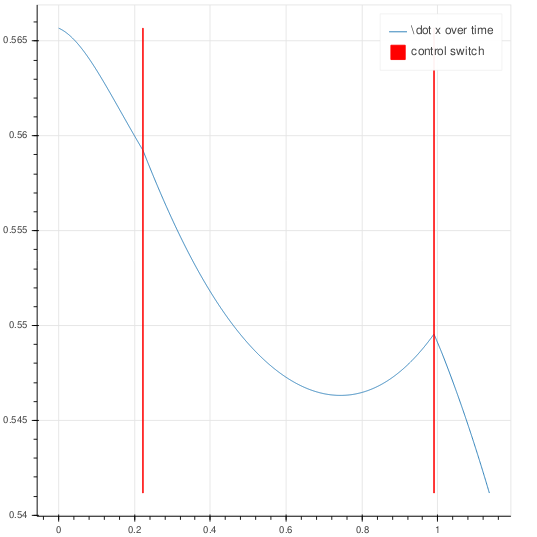
\includegraphics[width=.6\textwidth]{dotx}
\end{center}

\section{Заключение}
В ходе лабораторной работы применили метод малого параметра к задаче полёта на
максимальную дальность.

\printbibliography[title={Список литературы},heading=bibintoc]
\end{document}